\section{Optische Apparaturen}

\subsection{Abbildungssysteme -- Auge}

\subsubsection{Terminologie des Auges}

\paragraph{Sehwinkel $\varepsilon$}

\begin{minipage}{0.48\columnwidth}
    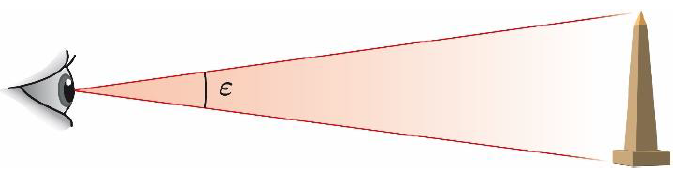
\includegraphics[width=0.9\columnwidth]{images/sehwinkel.png}
\end{minipage}
\hfill
\begin{minipage}{0.48\columnwidth}
    Die Grösse, in der ein Gegenstand dem betrachtenden Auge erscheint \textbf{(in Bogenminuten)} $\cbl{1 \degree \Leftrightarrow\ 60'}$
\end{minipage}


\medskip

\para{Auflösung}

Minimaler Winkelabstand $\varepsilon _{\rm min}$, den zwei Punkte haben müssen, damit sie noch getrennt wahrgenommen werden. \\
Normalsichtiges Auge: Auflösung ca. 1 Bogenminute ($1'$)

\medskip


\para{Sehschärfe}

Reziprokwert der Auflösung

$$ \boxed{ S = \frac{1}{\varepsilon _{\rm min}} \qquad \text{beim Menschen also } S = 1  } $$ 


\medskip

\paragraph{Deutliche Sehweite $\bm{s}$ (normierte Betrachtungsdistanz)}

Damit die Vergrösserungen von Lupen und Mikroskopen eindeutig bestimmt werden können, wird eine \textbf{deutliche Sehweite} definiert:

$$ \boxed{ s = 25 \, \mathrm{cm} = 0.25 \, \mathrm{m}  } $$ 


\subsubsection{Kurzsichtigkeit vs. Weitsichtigkeit}

\begin{minipage}{0.48\columnwidth}
    \raggedright
    \textbf{Kurzsichtigkeit} 

    \begin{itemize}
        \item Augapfel zu lang
        \item Konkave Streulinse als\\
            Korrektur
        \item Brille rückt Gegenstand näher heran 
    \end{itemize}
\end{minipage}
\hfill
\begin{minipage}{0.48\columnwidth}
    \raggedright
    \textbf{Weitsichtigkeit}

    \begin{itemize}
        \item Augapfel zu kurz
        \item Konvexe Sammellinse als Korrektur
        \item Brille rückt Gegenstand weiter weg 
    \end{itemize}
\end{minipage}


\subsection{Abbildungssysteme -- Fotoapparat}


\begin{minipage}{0.66\columnwidth}
    \paragraph{Bildgrösse $\bm{B}$} 

    Die Bildweite $b$ ist normalerweise viel kleiner als die
    Gegenstandsweite $g$ und daraus folgt:
\end{minipage}
\hfill
\begin{minipage}{0.3\columnwidth}
    $$ \boxed{ B = \frac{f}{g} \, G }$$
\end{minipage}

\smallskip


\begin{minipage}{0.66\columnwidth}
    \paragraph{Lichtstärke $\bm{H}$} 

    Die Intensität des Lichts auf dem Film ist gegeben durch
\end{minipage}
\hfill
\begin{minipage}{0.3\columnwidth}
    $$ \boxed{ H = \left(  \frac{d}{f} \right)^2 = q^2 } $$
\end{minipage}

\smallskip


\begin{minipage}{0.66\columnwidth}
    \paragraph{Blendenzahl $\bm{Z}$} 
    z.B.: 1, 1.4, 2, 2.8, 4, 5.6, \ldots
\end{minipage}
\hfill
\begin{minipage}{0.3\columnwidth}
    $$ \boxed{ Z = \frac{1}{q} = \frac{1}{\sqrt{H}}  } $$
\end{minipage}


\smallskip

\paragraph{Belichtung $\bm{E}$, Belichtungszeit $\bm{t}$} 

\begin{minipage}{0.66\columnwidth}
    $$ \boxed{ E = H t \approx q^2 t} $$
\end{minipage}
\hfill
\begin{minipage}{0.3\columnwidth}
    $$ \boxed{ t = \frac{G}{v} = \frac{g}{f} \frac{B}{v} } $$
\end{minipage}




\smallskip

\paragraph{Schärfentiefe} 

In der Filmebene ergibt sich vom Punkt $G$ kein scharfer Bildpunkt, sondern ein \textbf{Unschärfekreis} mit dem Durchmesser $u$. 

Es wird folgende Gegenstandsweite $g$ in den Unschärfekreis abgebildet:

\begin{minipage}{0.65\columnwidth}
    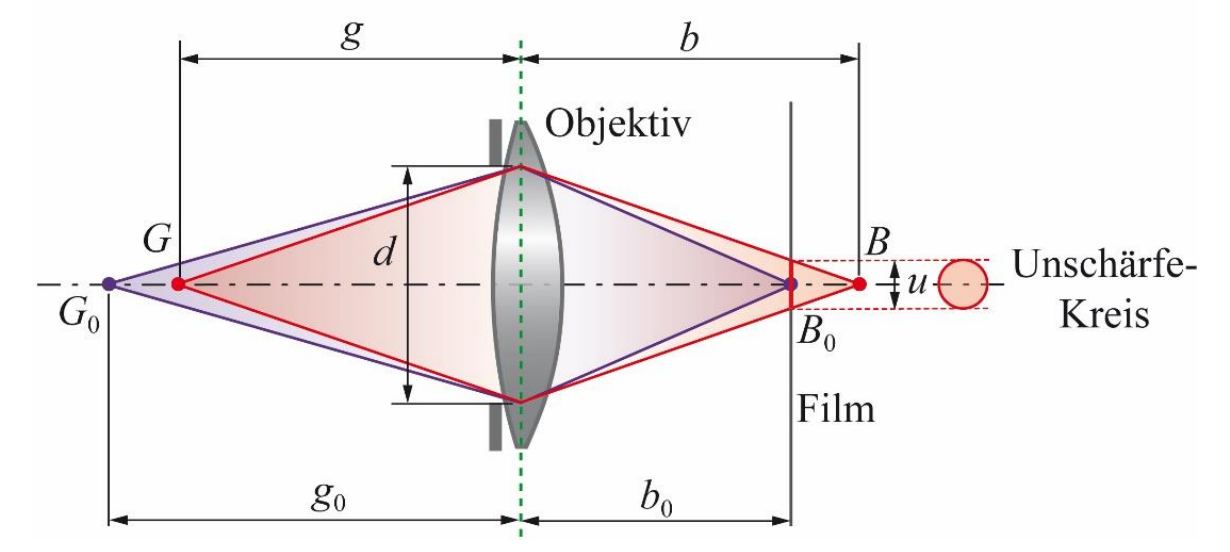
\includegraphics[width=\columnwidth]{images/schaerfentiefe.png}
\end{minipage}
\hfill
\begin{minipage}{0.3\columnwidth}
    $$\boxed{ \frac{1}{g} = \frac{1}{g_0} \pm \frac{u}{q \, f^2}  } $$
\end{minipage}

\begin{ctabular}{c l c}
	$b$     & Bildweite                                             & $[b] = \meter$    \\
	$b_0$   & $\text{Bilddlistanz}_0$                               & $[b_0] = \meter$  \\
	$B$     & $\text{Bildgrösse}$                                   & $[B] = \meter$    \\
	$B_0$   & $\text{Bild}_0$                                       & $[B_0] = \meter$  \\
	$g$     & Gegenstandsweite ($G$ zu Objektiv)                    & $[g] = \meter$    \\
	$g_0$   & $\text{Gegenstandsdistanz}_0$ ($G_0$ zu Objektiv)     & $[g_0] = \meter$  \\
	$G$     & Gegenstandsgrösse                                     & $[G] = \meter$    \\
	$G_0$   & $\text{Gegenstandsgrösse}_0$                          & $[G_0] = \meter$  \\
	$f$     & Brennweite                                            & $[f] = \meter$    \\
	$u$     & Durchmesser Unschärfekreis                            & $[u] = \meter$    \\
	$d$     & Durchmesser Blendenöffnung                            & $[d] = \meter$
\end{ctabular}


\subsection{Abbildungssysteme -- Lupe}

\begin{minipage}{0.48\columnwidth}
    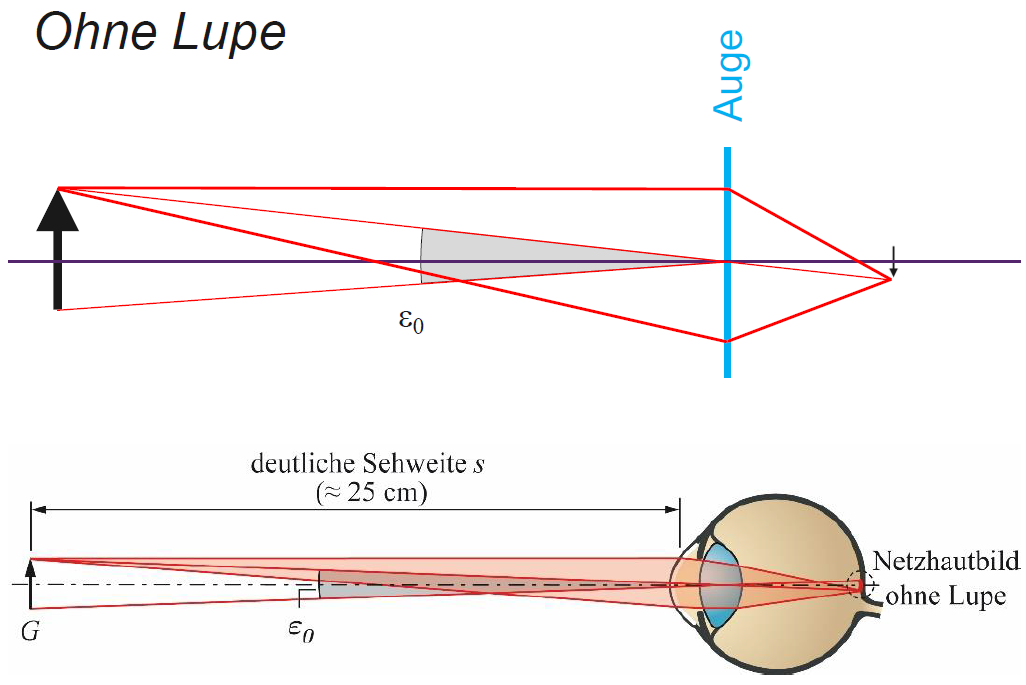
\includegraphics[width=0.9\columnwidth]{images/ohne_lupe.png}

    $$ \boxed{ \tan(\varepsilon_0) = \frac{G}{s} } $$
\end{minipage}
\hfill
\begin{minipage}{0.48\columnwidth}
    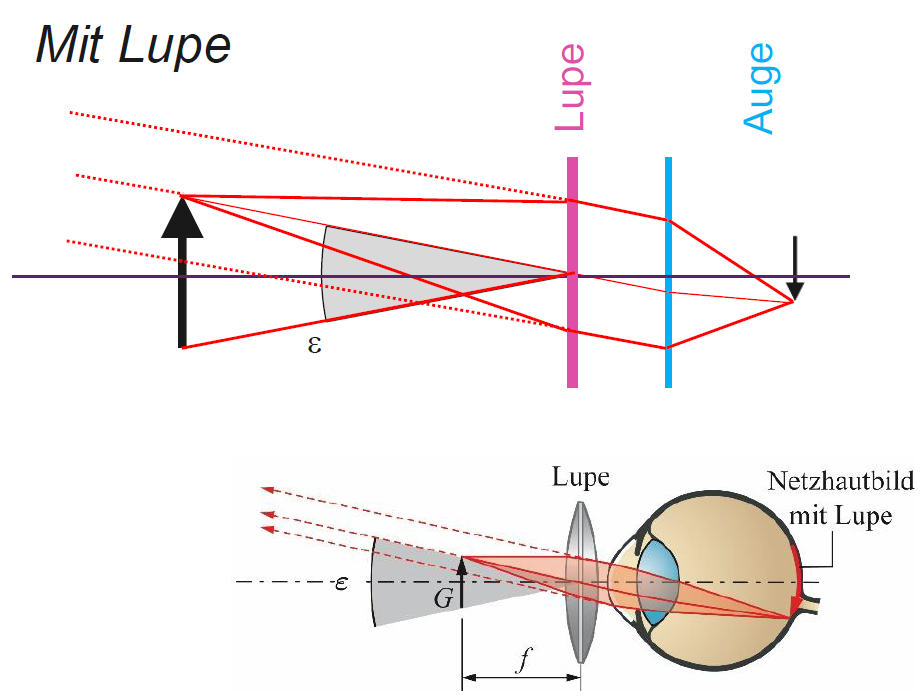
\includegraphics[width=0.9\columnwidth]{images/mit_lupe.png}

    $$ \boxed{ \tan(\varepsilon) = \frac{G}{f} } $$
\end{minipage}

$$ \boxed{ V = \frac{\tan(\varepsilon)}{\tan(\varepsilon_0)} = \frac{s}{f} } $$

\begin{ctabular}{c l c}
	$\varepsilon_i$ & Sehwinkel                                 & $[\varepsilon_i] = \degree$   \\
	$s$             & Deutliche Sehweite $s =0.25 \, \meter$    & $[s] = \meter$                \\
	$f$             & Brennweite                                & $[f] = \meter$                \\
	$V$             & Vergrösserung                             & $[V] = 1$                     \\
    $G$             & Gegenstandsgrösse                         & $[G] = \meter$                
\end{ctabular}


\subsection{Abbildungssysteme -- Fernrohr}

Es wird zuerst ein vergrössertes Bild erzeugt, welchs selber wiederum mit einer Lupe betrachtet wird.

\begin{center}
    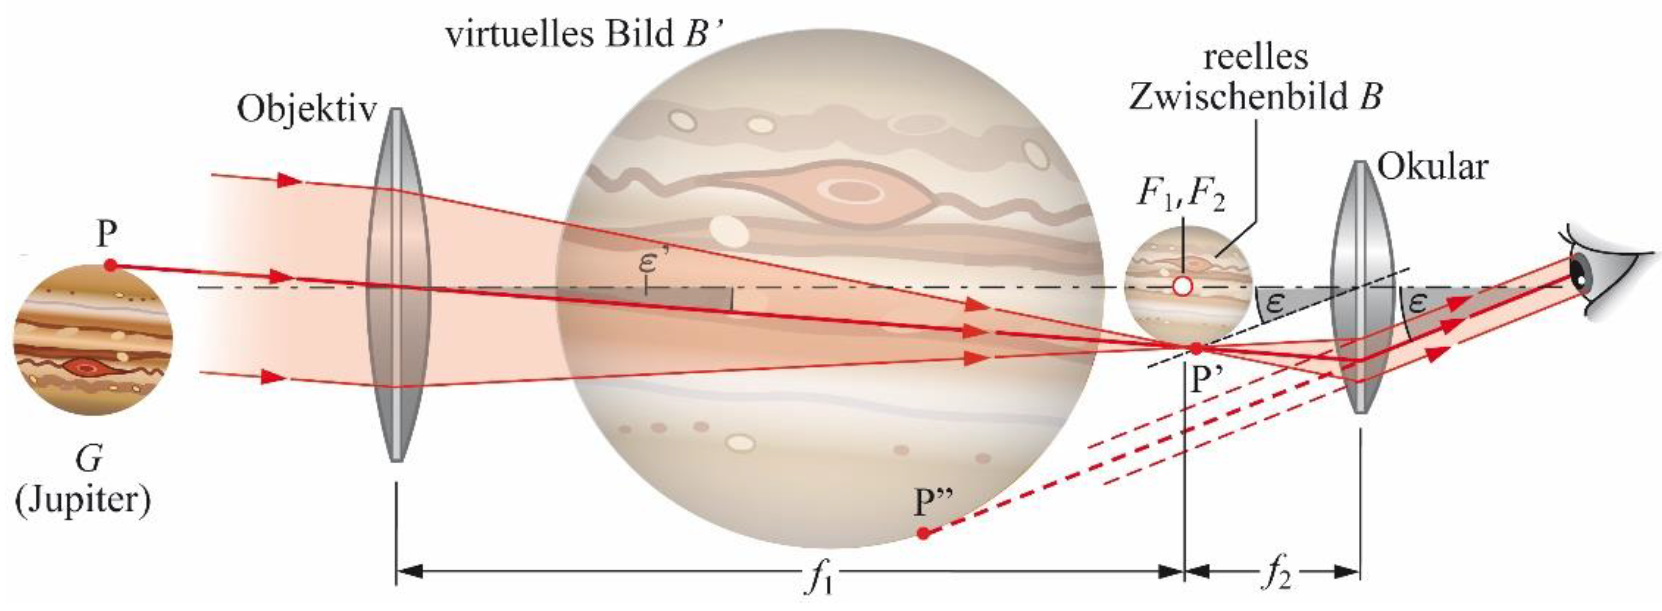
\includegraphics[width=0.9\columnwidth]{images/fernrohr.png}
\end{center}

\begin{minipage}[c]{0.48\columnwidth}
    $$ \boxed{ V = \frac{\tan(\varepsilon)}{\tan(\varepsilon_0)} = \frac{\frac{B}{f_2}}{\frac{B}{f_1} } = \frac{f_1}{f_2} } $$
\end{minipage}
\hfill
\begin{minipage}[c]{0.48\columnwidth}
    \begin{ctabular}{c l c}
        $\varepsilon_i$     & Sehwinkel                                     & $[\varepsilon_i] = \degree$   \\
        $f_i$               & Brennweite                                    & $[f_i] = \meter$              \\
        $V$                 & Vergrösserung                                 & $[V] = 1$                     \\
        $B$                 & Bildgrösse                                    & $[B] = \meter$                
    \end{ctabular}
\end{minipage}

\columnbreak


\subsection{Abbildungssysteme -- Mikroskop}

Es wird zuerst ein vergrössertes Bild erzeugt, welchs selber wiederum mit einer Lupe betrachtet wird. 

\medskip
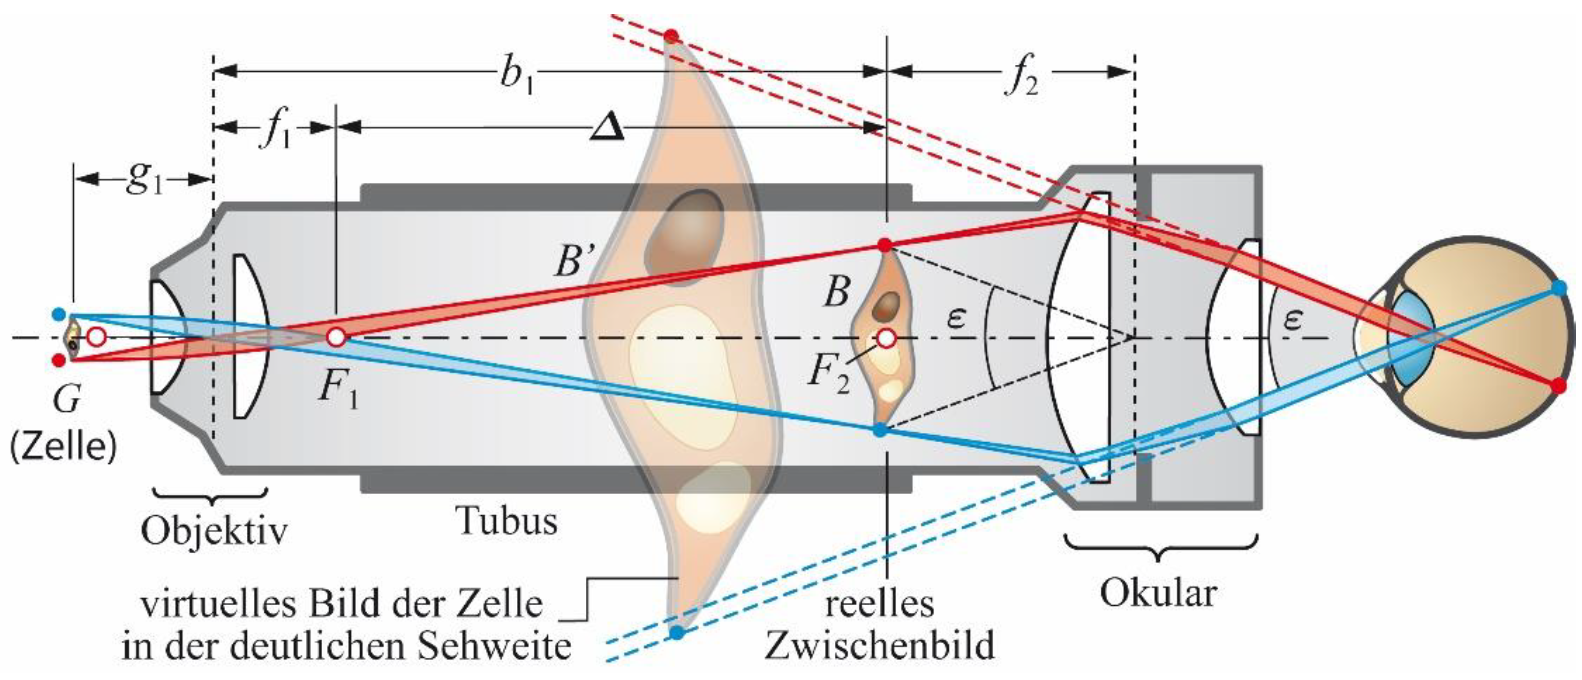
\includegraphics[width=0.9\columnwidth]{images/mikroskop.png}

$$ \boxed{ V = \underbrace{ \frac{\Delta}{f_1} }_{V_1} \cdot \underbrace{ \frac{s}{f_2} }_{V_2} = \frac{\tan(\varepsilon)}{\tan(\varepsilon_0)} = \frac{\frac{B}{f_2}}{\frac{G}{s}} = \frac{B}{G} \frac{s}{f_2} = \frac{b_1}{g_1} \frac{s}{f_2} } $$

\begin{ctabular}{c l c}
	$\varepsilon_i$     & Sehwinkel                                     & $[\varepsilon_i] = \degree$   \\
	$s$                 & Deutliche Sehweite $s =0.25 \, \meter$        & $[s] = \meter$                \\
	$f_i$               & Brennweite                                    & $[f_i] = \meter$              \\
	$V$                 & Vergrösserung                                 & $[V] = 1$                     \\
	$\Delta$            & optische Tubuslänge (Abstand der Brennpunkte) & $[\Delta] = \meter$           \\
	$b_1$               & Bildweite                                     & $[b_1] = \meter$              \\
	$g_1$               & Gegenstandsweite                              & $[g_1] = \meter$              \\
	$B$                 & Bildgrösse                                    & $[B] = \meter$                \\
	$G$                 & Gegenstandsgrösse                             & $[G] = \meter$
\end{ctabular}


\subsection{Farbentheorie}

\begin{description}
    \item[Spektralfarben:] Die gesamten Lichtfarben
    \item[Monochromatisches Licht:] Nur eine einzige Wellenlänge (Farbe) 
\end{description}


\subsubsection{Farbmischungen}

\begin{minipage}{0.42\columnwidth}
    \textbf{Additive Farbmischung}

    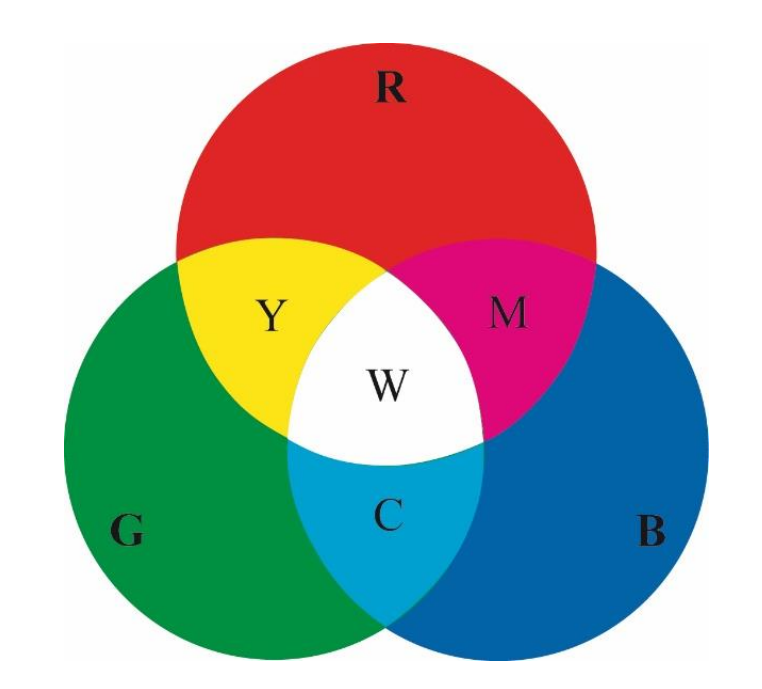
\includegraphics[width=\columnwidth]{images/additiveFarbmischung.png}
\end{minipage}
\hfill
\begin{minipage}{0.42\columnwidth}
    \textbf{Subtraktive Farbmischung}

    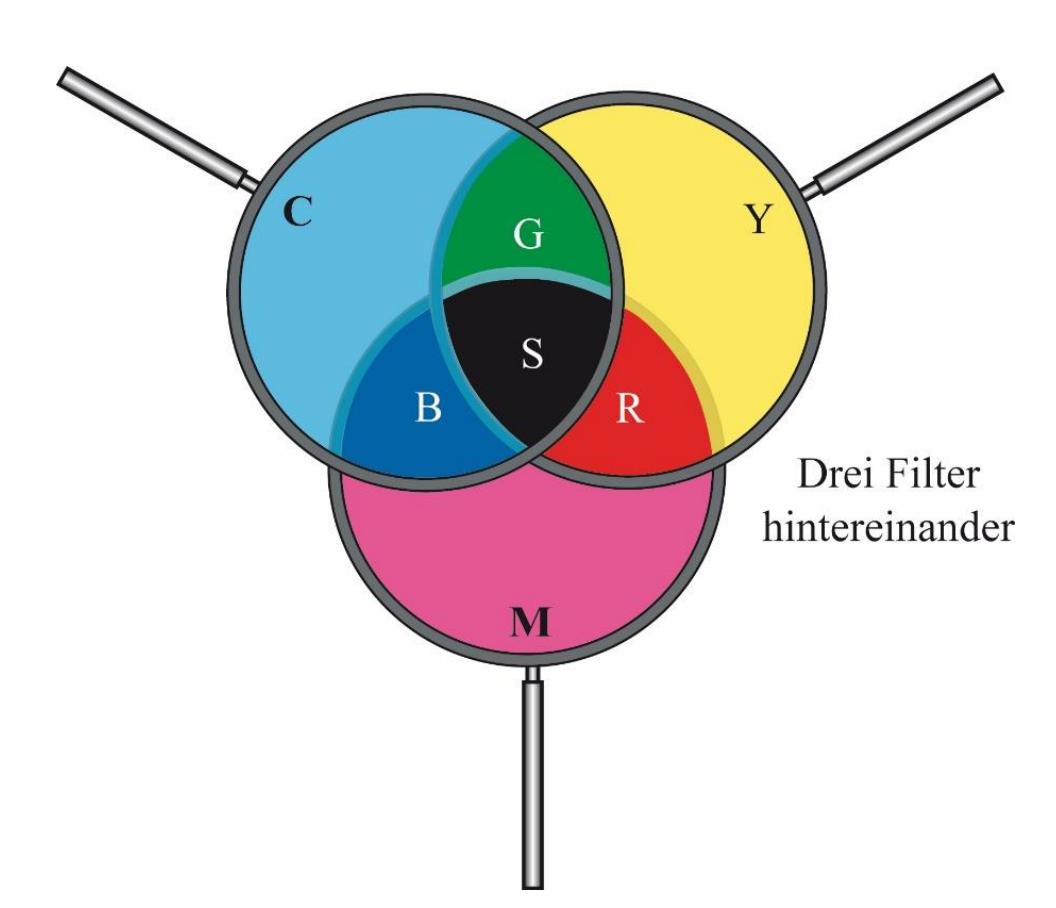
\includegraphics[width=\columnwidth]{images/SubtraktiveFarbmischung.png}
\end{minipage}

